\chapter{L'Entreprise --- Société Régionale Multiservices Souss-Massa}

\section{Cadre Légal et Genèse}
La création des Sociétés Régionales Multiservices (SRM) résulte de la réforme nationale de la gestion des services publics locaux de distribution d'eau, d'électricité et d'assainissement liquide, portée par la \textbf{loi n° 83-21}.
\begin{itemize}
    \item \textbf{Adoption :} 12 juin 2023 (Chambre des Représentants).
    \item \textbf{Promulgation :} dahir n° 1-23-53 du 12 juillet 2023.
    \item \textbf{Publication :} Bulletin Officiel n° 7213 du 17 juillet 2023.
    \item \textbf{Objectif de la réforme :} régionaliser et unifier la gestion de l'eau, de l'électricité et de l'assainissement, jusque-là fragmentée entre régies autonomes municipales (RAMSA, RADEEMA, RADEEF, etc.), concessionnaires privés (Lydec, Amendis) et l'ONEE, en une société unique par région administrative, sous tutelle conjointe de l'État et des collectivités territoriales.
\end{itemize}

La \textbf{SRM Souss-Massa} est entrée en activité le \textbf{15 octobre 2024}, dans le cadre de la première vague de déploiement (avec les SRM de l'Oriental, de Casablanca-Settat et de Marrakech-Safi). Elle succède à la \textbf{RAMSA} (Régie Autonome Multi-Services d'Agadir), dont elle reprend le patrimoine, le personnel et les systèmes d'information existants.

\IfFileExists{images/img_004_chronologie_loi_83_21_creation.png}{%
\begin{figure}[H]
    \centering
    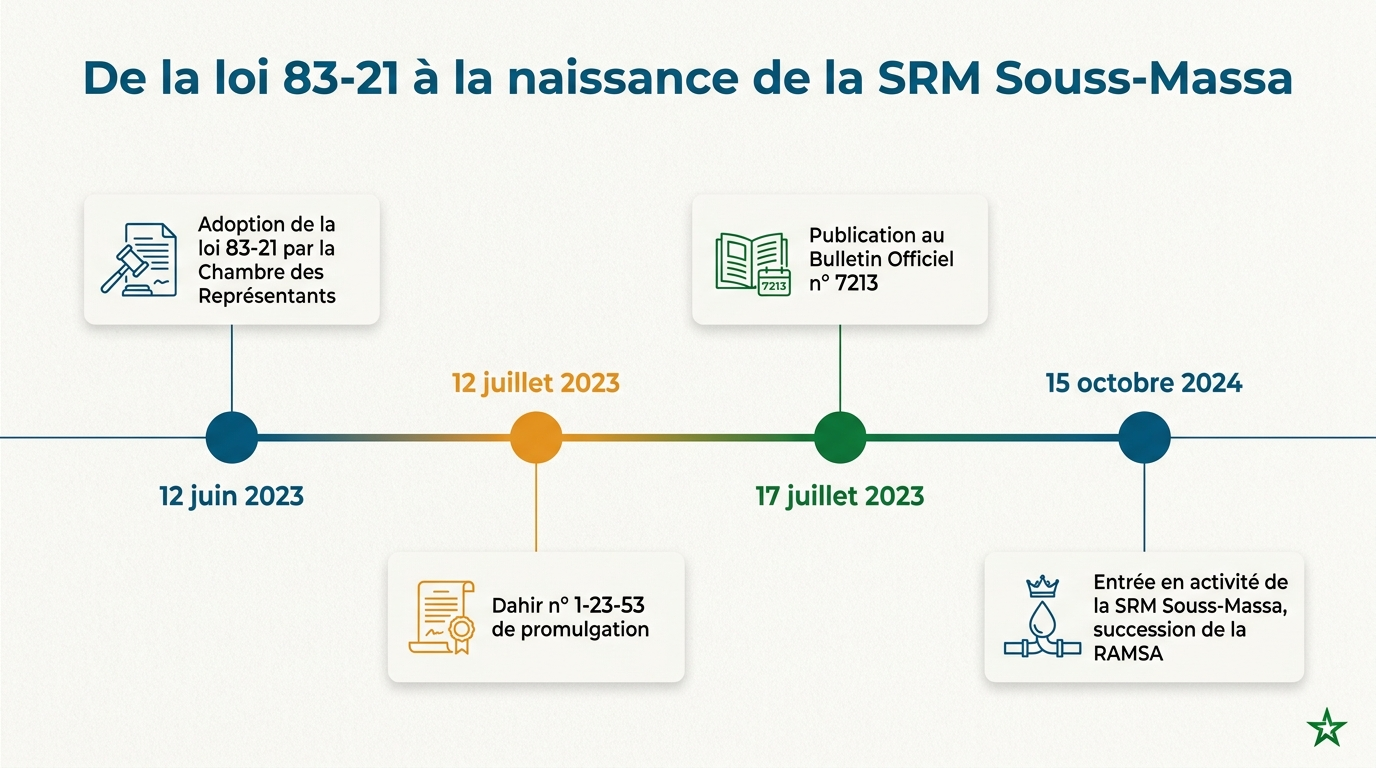
\includegraphics[width=\textwidth]{images/img_004_chronologie_loi_83_21_creation.png}
    \caption{De la loi 83-21 à la naissance de la SRM Souss-Massa}
\end{figure}}{}

\section{Périmètre Géographique et Missions}
Le périmètre de la SRM Souss-Massa couvre l'intégralité de la région Souss-Massa :
\begin{itemize}
    \item \textbf{Deux préfectures :} Agadir Ida-Outanane, Inezgane Aït Melloul.
    \item \textbf{Quatre provinces :} Chtouka-Aït Baha, Taroudant, Tiznit, Tata.
    \item \textbf{175 communes}, pour une population d'environ \textbf{3,06 millions d'habitants}.
\end{itemize}

Ses missions, exercées en \textbf{guichet unique}, sont :
\begin{enumerate}
    \item la production et la distribution d'\textbf{eau potable} ;
    \item la distribution d'\textbf{électricité} (moyenne et basse tension) ;
    \item l'\textbf{assainissement liquide} (collecte et épuration des eaux usées) ;
    \item l'\textbf{éclairage public}.
\end{enumerate}

\IfFileExists{images/img_005_perimetre_geographique_srm.png}{%
\begin{figure}[H]
    \centering
    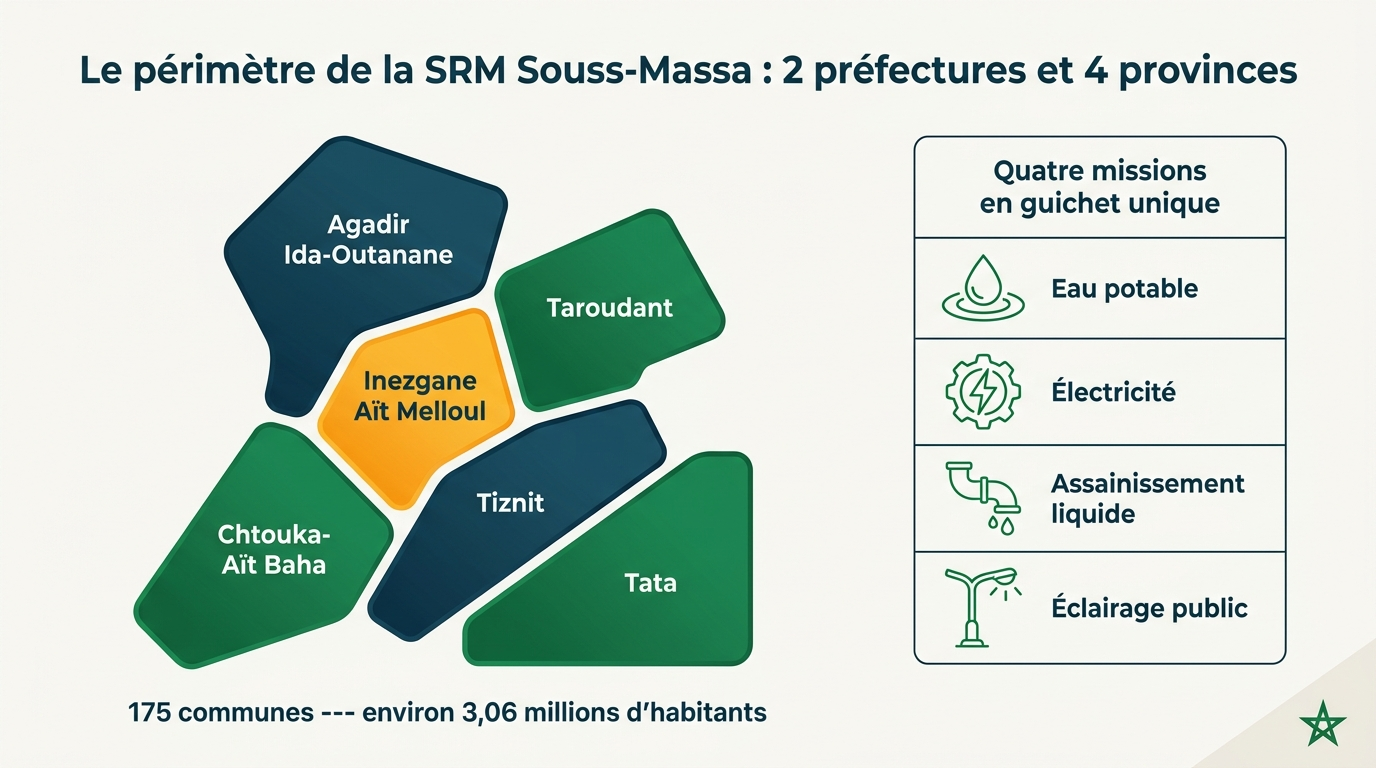
\includegraphics[width=\textwidth]{images/img_005_perimetre_geographique_srm.png}
    \caption{Le périmètre de la SRM Souss-Massa : 2 préfectures et 4 provinces}
\end{figure}}{}

\section{Gouvernance et Actionnariat}
La SRM Souss-Massa est une société anonyme à conseil d'administration, à capitaux 100 \% publics.
\begin{itemize}
    \item \textbf{Président du Conseil d'Administration :} Saaïd Amzazi (Wali de la région Souss-Massa).
    \item \textbf{Directeur Général :} Mohamed Amrzak.
    \item \textbf{Structure de l'actionnariat} (répartition type des SRM issues de la réforme) : État (environ 40 \%), Région (environ 25 \%), communes urbaines et rurales regroupées (environ 25 \%), et une part résiduelle (environ 10 \%) selon les conventions locales de transfert d'actifs.
\end{itemize}

\IfFileExists{images/img_006_gouvernance_actionnariat_srm.png}{%
\begin{figure}[H]
    \centering
    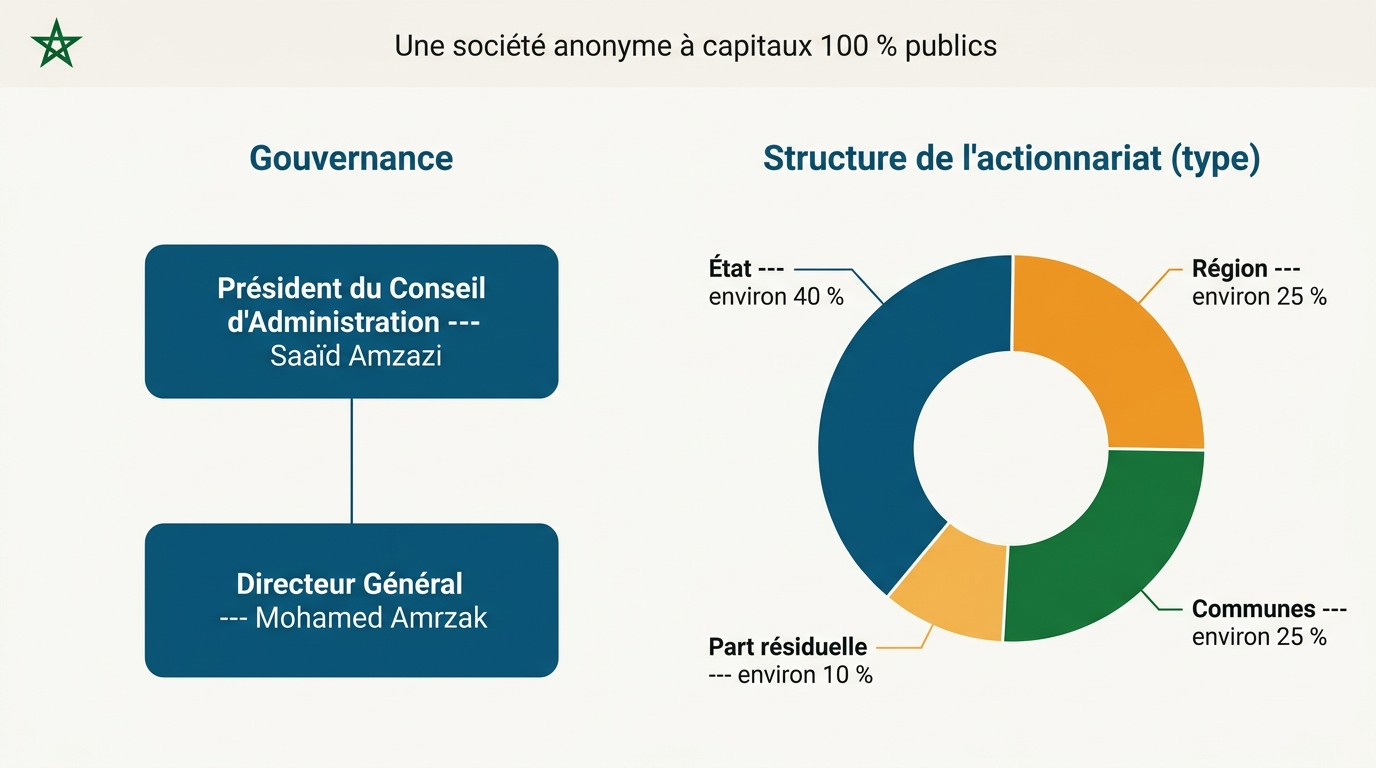
\includegraphics[width=0.9\textwidth]{images/img_006_gouvernance_actionnariat_srm.png}
    \caption{Une société anonyme à capitaux 100 \% publics : gouvernance et actionnariat}
\end{figure}}{}

\begin{tcolorbox}[colback=blue!4!white,colframe=blue!40!black,title=\textbf{Chiffres clés à mémoriser}]
\begin{itemize}
    \item \textbf{Budget d'investissement annoncé :} environ \textbf{19,68 milliards de dirhams} sur 30 ans, dont un plan quinquennal \textbf{2025--2029}.
    \item \textbf{Stress hydrique :} la région Souss-Massa fait partie des régions marocaines les plus touchées par le stress hydrique structurel, ce qui place les projets de \textbf{dessalement d'eau de mer} au cœur de la stratégie régionale.
    \item \textbf{Projet de dessalement de Chtouka-Aït Baha :} déjà opérationnel, alimente notamment l'irrigation agricole et l'eau potable de la zone.
    \item \textbf{Méga-projet Tiznit--Chtouka :} annoncé le 27 août 2026, nouveau projet structurant de dessalement/transfert d'eau pour sécuriser l'approvisionnement de la région.
    \item \textbf{Barrage Tamri :} ouvrage régional participant à la sécurisation de la ressource en eau de la province d'Agadir Ida-Outanane.
\end{itemize}
\end{tcolorbox}

\IfFileExists{images/img_007_stress_hydrique_projets_dessalement.png}{%
\begin{figure}[H]
    \centering
    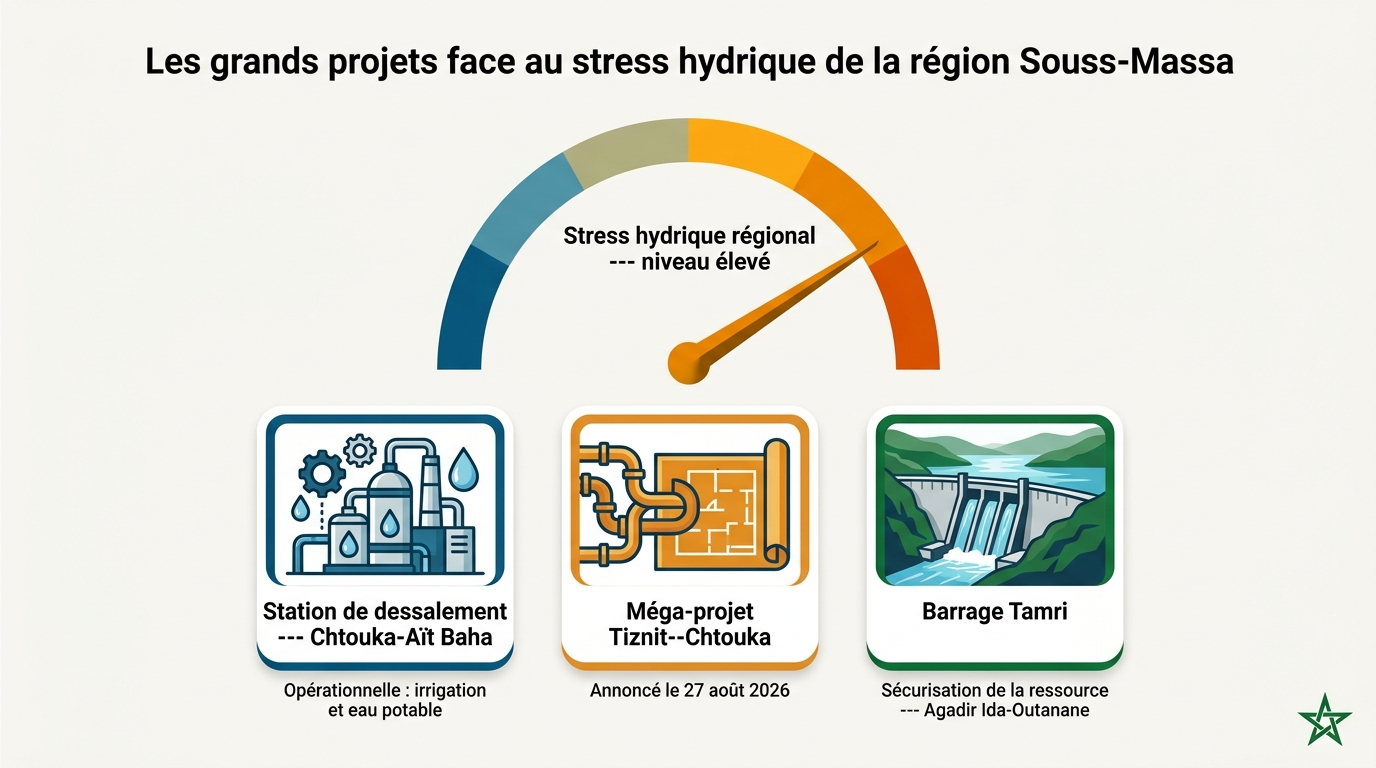
\includegraphics[width=\textwidth]{images/img_007_stress_hydrique_projets_dessalement.png}
    \caption{Les grands projets face au stress hydrique de la région Souss-Massa}
\end{figure}}{}

\section{Les Autres SRM Créées en 2026 --- Repères de Comparaison}
La réforme s'est poursuivie en 2026 avec la création de nouvelles SRM, dont les effectifs de recrutement donnent une idée de l'ampleur de la réforme nationale :
\begin{table}[H]
\centering
\small
\begin{tabular}{|p{5cm}|p{8.5cm}|}
\hline
\rowcolor{gray!20} \textbf{SRM} & \textbf{Repère} \\ \hline
SRM Fès-Meknès & environ 39 postes ouverts au recrutement 2026 \\ \hline
SRM Casablanca-Settat & plus de 1000 postes ouverts (plus grande région économique du pays) \\ \hline
SRM Rabat-Salé-Kénitra & environ 356 postes ouverts \\ \hline
SRM Drâa-Tafilalet & environ 140 postes ouverts \\ \hline
SRM de l'Oriental & une des quatre SRM de la première vague (2024), comme la SRM Souss-Massa \\ \hline
\end{tabular}
\caption{Ordres de grandeur des recrutements SRM 2026 (à titre de repère de culture générale, non un fait à réciter pour la SRM Souss-Massa elle-même)}
\end{table}

\IfFileExists{images/img_013_comparatif_srm_2026.png}{%
\begin{figure}[H]
    \centering
    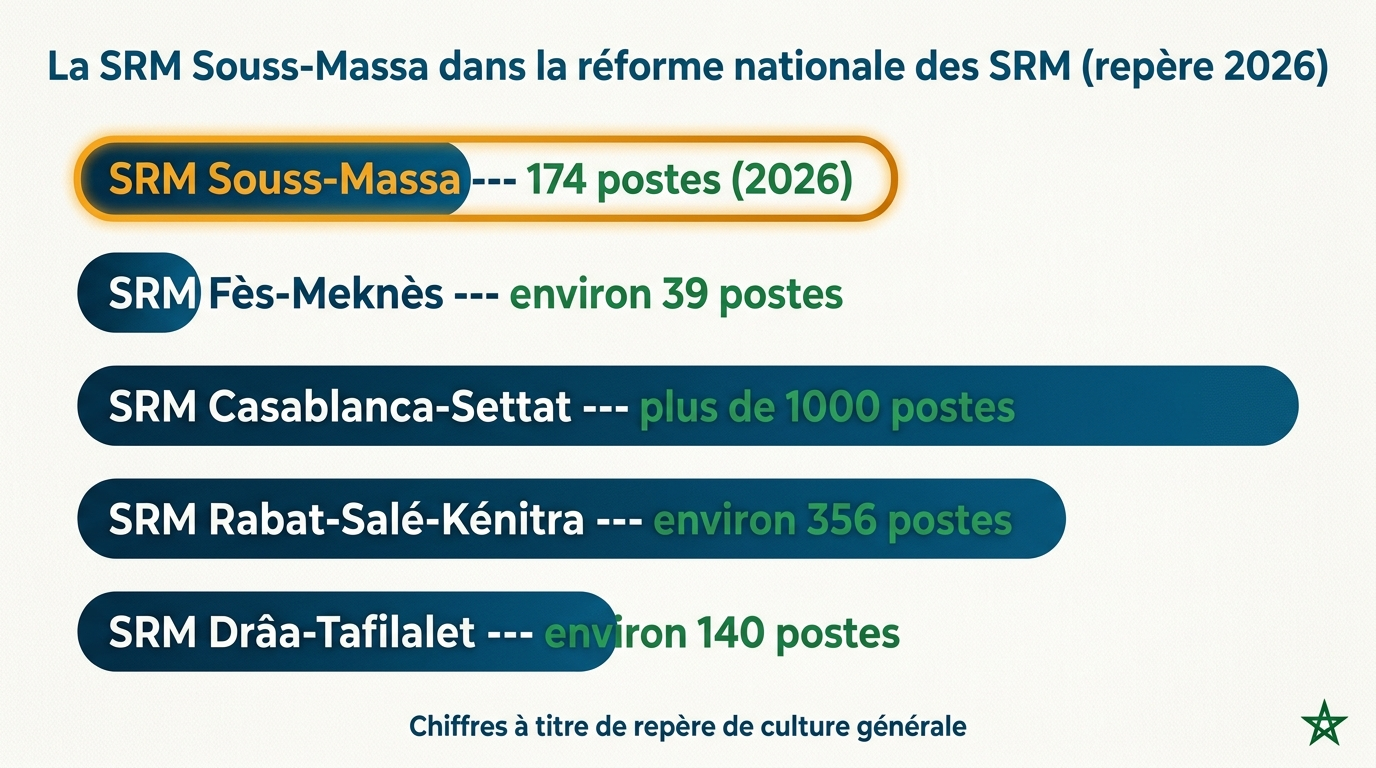
\includegraphics[width=\textwidth]{images/img_013_comparatif_srm_2026.png}
    \caption{La SRM Souss-Massa dans la réforme nationale des SRM (repère 2026)}
\end{figure}}{}

\section{Le Recrutement 2026 de la SRM Souss-Massa}
L'avis de recrutement (code concours \textbf{C43190/26}, publié le \textbf{7 août 2026} sur \texttt{emploi-public.ma}, organisme recruteur \textbf{Brain Management}) ouvre \textbf{174 postes} au total, répartis en quatre concours distincts :
\begin{itemize}
    \item \textbf{9 cadres expérimentés} (entretien oral seul, sans épreuve écrite).
    \item \textbf{38 cadres techniques Bac+5 / ingénieurs d'État} (écrit puis oral) --- \textbf{c'est votre concours}, spécialités GI / SI / RT / IA \& DATA / GL / CYBER, poste rattaché à la \textbf{Direction Centrale}.
    \item \textbf{64 agents de maîtrise}.
    \item \textbf{63 agents d'exécution}.
\end{itemize}

\begin{tcolorbox}[colback=blue!4!white,colframe=blue!40!black,title=\textbf{Votre catégorie précisément : 6 postes sur 38}]
Selon la fiche technique de l'avis (répartition par spécialité des 38 postes \og cadres \fg{}) : 12 postes en génie de l'eau/électricité/civil/environnement, \textbf{6 postes en informatique/cyber/data} (\textbf{votre spécialité}), 10 postes de gestion (audit, finance, RH, comptabilité), 8 postes commerciaux/marketing/juridiques, 2 postes QSE/efficacité énergétique. Répartition géographique des 38 postes : 28 pour Agadir Ida-Outanane/Direction Centrale, 5 à 6 pour Taroudant, 2 pour Tata, 1 à 2 pour Tiznit, 1 pour Inezgane Aït Melloul (les sources diffèrent légèrement sur ce dernier détail).
\end{tcolorbox}

\textbf{Conditions d'âge :} être âgé de 18 ans au moins et \textbf{40 ans au plus} au 31 décembre 2026 pour la catégorie cadres (45 ans pour les cadres expérimentés, 35 ans pour les agents d'exécution). \textbf{Diplôme requis :} diplôme d'Ingénieur d'État, Master ou Grande École (Bac+5) dans la spécialité, avec attestation d'équivalence si diplôme étranger ou d'établissement privé.

\IfFileExists{images/img_008_recrutement_2026_174_postes.png}{%
\begin{figure}[H]
    \centering
    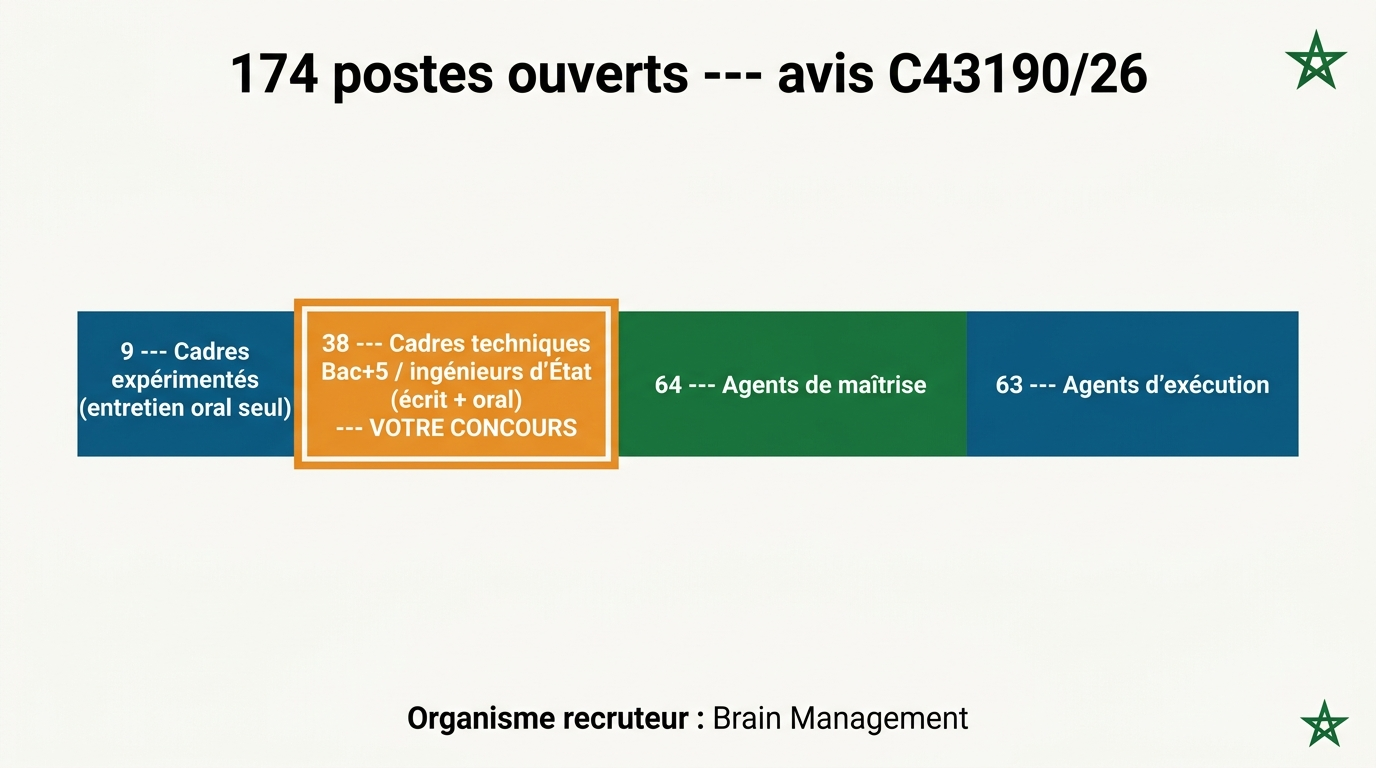
\includegraphics[width=\textwidth]{images/img_008_recrutement_2026_174_postes.png}
    \caption{174 postes ouverts --- avis C43190/26}
\end{figure}}{}

\section{Pourquoi ces Repères Comptent pour le QCM}
Les questions de culture générale et entreprise du QCM portent typiquement sur des faits vérifiables et datés : la base légale (loi 83-21, dahir, date de publication au BO), la date de création effective de la SRM Souss-Massa, son périmètre géographique exact, ses missions, sa gouvernance, et les grands projets structurants (dessalement, barrages) liés au contexte de stress hydrique régional. Mémoriser ces repères avec leurs dates et chiffres précis, plutôt que leur seule idée générale, est la stratégie la plus rentable pour ce bloc du QCM.
